Random forest là một phương pháp thống kê mô hình hóa bằng máy (Machine learning statistic) dùng để phục vụ các mục đích phân loại, tính hồi quy và các nhiệm vụ khác bằng cách xây dựng nhiều cây quyết định (Decision tree). Một cây quyết định là một cách đơn giản để biểu diễn một giao thức. Nói cách khác, cây quyết định biểu diễn một kế hoạch, trả lời câu hỏi phải làm gì trong một hoàn cảnh nhất định.

\begin{figure}[htbp]
\centerline{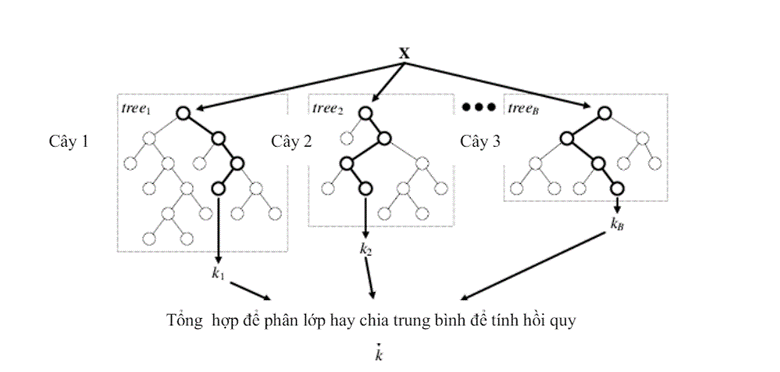
\includegraphics[width=0.4\textwidth]{img/RF.png}}
\caption{Sơ đồ biểu diễn các cây quyết định trong Random Forest}
\label{fig}
\end{figure}

Mỗi node của cây sẽ là các thuộc tính, và các nhánh là giá trị lựa chọn của thuộc tính đó. Bằng cách đi theo các giá trị thuộc tính trên cây, cây quyết định sẽ cho ta biết giá trị dự đoán. Nhóm thuật toán cây quyết định có một điểm mạnh đó là có thể sử dụng cho cả bài toán phân loại và hồi quy. Do đó, Random Forest có thể được sử dụng vào các nghiên cứu phân tích và dự báo chuỗi thời gian. Random Forest có khả năng tìm ra thuộc tính nào quan trọng hơn so với những thuộc tính khác. Trên thực tế, nó còn có thể chỉ ra rằng một số thuộc tính là không có tác dụng trong cây quyết định. Từ hình 7, chúng ta thấy rằng Random Forest được cấu thành bởi một số cây quyết định. Các cây này cùng nhận đầu vào là đối tượng x và đưa ra quyết định về danh mục thuộc tính của x. Các quyết định này sẽ được tổng hợp lại lấy trung bình để chọn ra quyết định cuối cùng.


